% Chapter 1

\chapter{Thoughts \& ideas} % Main chapter title

\label{sec:ideas} % For referencing the chapter elsewhere, use \ref{Chapter1} 

\section{Calibration over original inputs}

In the standard calibration procedure we change the transition probabilities in the matrices, assuming they are independent and enforcing constraints in the error calculation step. One alternative would be to calibrate over those relevant original inputs (i.e. those found in the literature, studies, expert opinions, ...) and then calculate the transition probabilities (and possibly other inputs of the model) from them. With this method we preserve and inject the knowledge we have about the domain into the model (that is, how to calculate the probabilities from the scientific sources, assumptions, implicit restrictions, ...).

\begin{figure}[h]
	\centering
	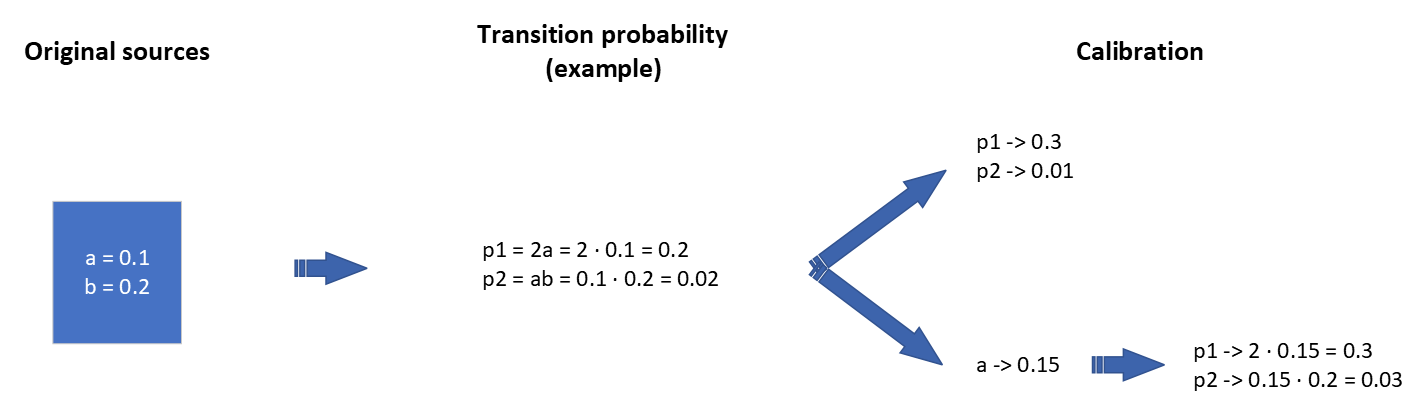
\includegraphics[width=\textwidth]{figures/calibration_inputs}
	\decoRule
	\caption[Calibration over inputs]{Calibration procedures: directly over the probabilities (``Calibration'', top) and over the original inputs (``Calibration'', bottom).}
	\label{fig:calibration_inputs}
\end{figure}

Since we calibrate to account for the uncertainty in the natural history and the probabilities in the matrices are calculated from parameters, we could classify the uncertainty sources in two: uncertainty associated to the inputs and uncertainty associated to the calculation of the probability.

\subsection{Parameter uncertainty}
If we are sure about the calculation of the transition probability, like a well-known relationship (e.g. Bayes formula), the remaining sources of uncertainty are the inputs themselves. In this case we can set up the optimizer to change these inputs, recalculate the probabilities and run the model.

For interpretation and sanity check purposes we can check both the changed input value and the newly-calculated transition probability.

\begin{figure}[h!]
	\centering
	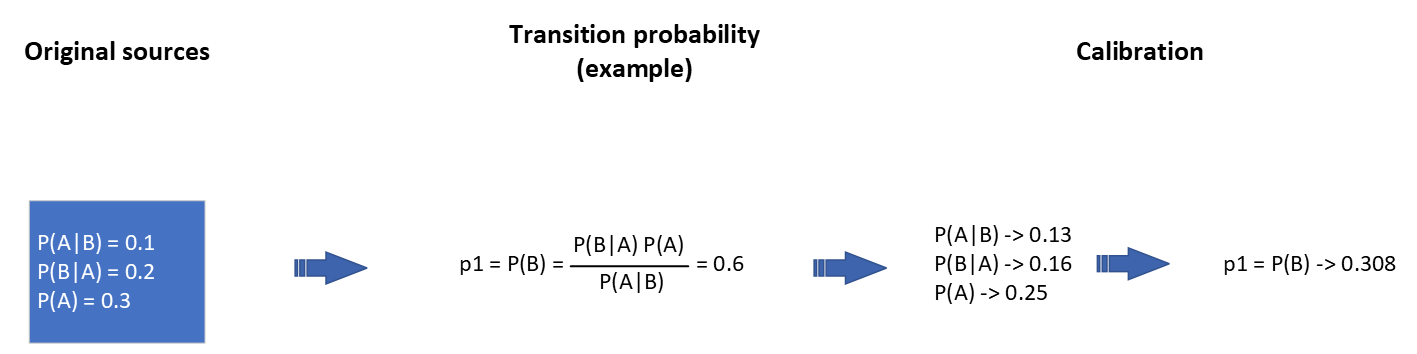
\includegraphics[width=\textwidth]{figures/calibration_values}
	\decoRule
	\caption[Calibration over input values]{If we are certain of the relationship between the probability and the inputs, we can calibrate over the inputs and we will get the calibrated probability by preserving the link with the original inputs.}
	\label{fig:calibration_values}
\end{figure}

\subsection{Calculation uncertainty}
Beyond the inputs, the calculation itself might be uncertain as well, for example by making a very rough approximation or assuming a probabilistic distribution with a poor fit. In this case we can insert an error term or scaling factor in the formula to account for the misspecification, with a neutral initial value (0 if error, 1 if factor). Then, the calibration could include these error/scaling terms in the set of parameters to be optimized.

For interpretation and sanity check purposes, besides the probabilities themselves as usual, we can check the error term/scaling factor. If they are too different from the initial values we might conclude that the calculation is not trustworthy and we might have to review our assumptions. Also, if the calculation is a very rough estimate another alternative would be to reject the calculation itself and optimize the probability value as usual.

\begin{figure}[h!]
	\centering
	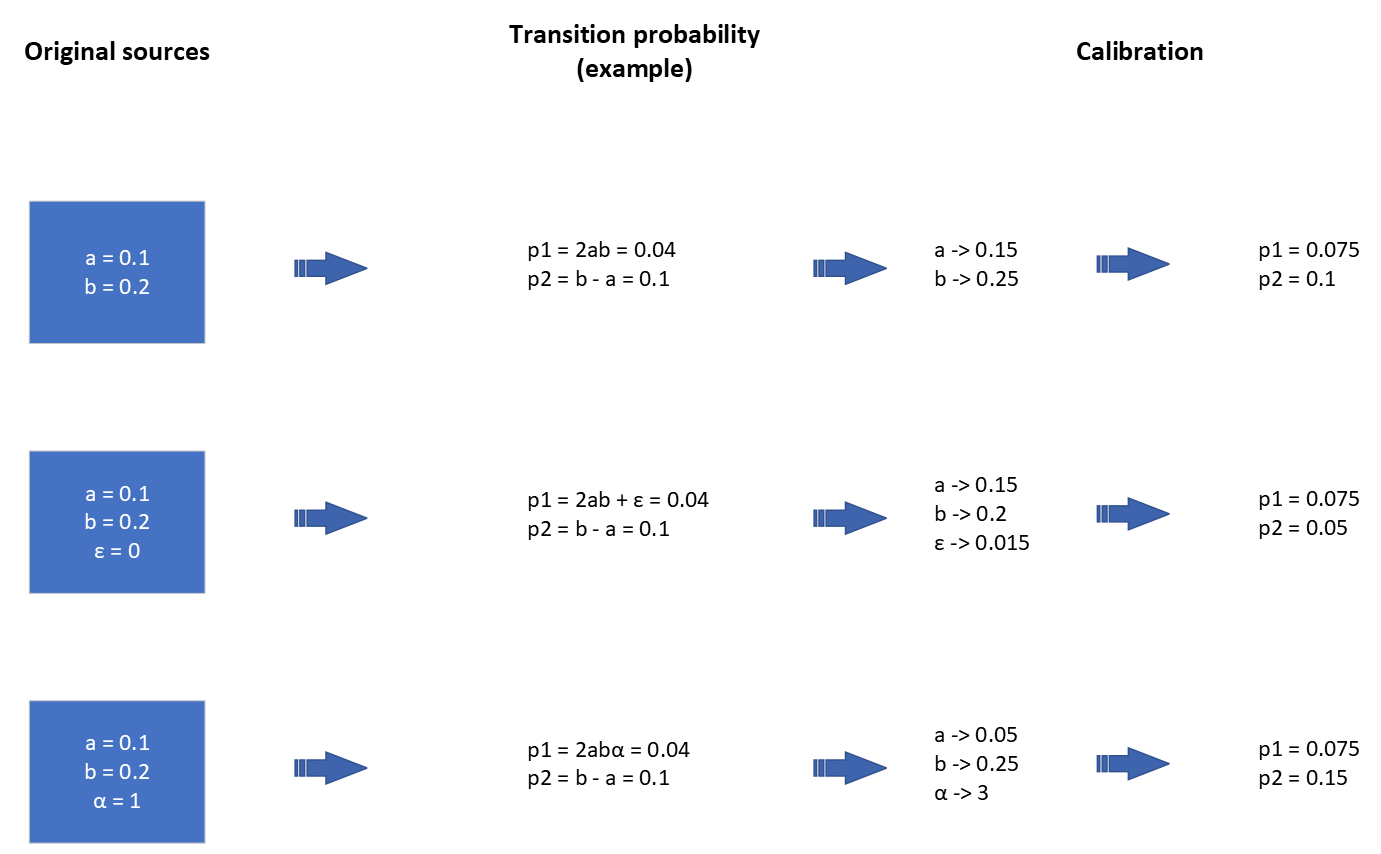
\includegraphics[width=\textwidth]{figures/calibration_calculation}
	\decoRule
	\caption[Calibration over calculations]{To account for the possibility of a misspecified calculation we can add additional terms to a formula. We can see calibration with no formula flexibility (top row), an additive error term for p1 (middle row) or a multiplicative factor for p1 (bottom row).}
	\label{fig:calibration_calculation}
\end{figure}

\subsection{Comments}

\subsubsection*{Pros}
\begin{itemize}
	\item Preserving the link and implicit knowledge between the original sources and the calculated probabilities
	\item Preserving relationships between probabilities and (some kinds of) constraints
\end{itemize}

\subsubsection*{Cons}
\begin{itemize}
	\item Overcomplicating the calibration procedure in simple cases
	\item Relationships might not be too complicated
\end{itemize}

\section{Input/probabilities dependencies using graph theory}

\begin{figure}[h!]
	\centering
	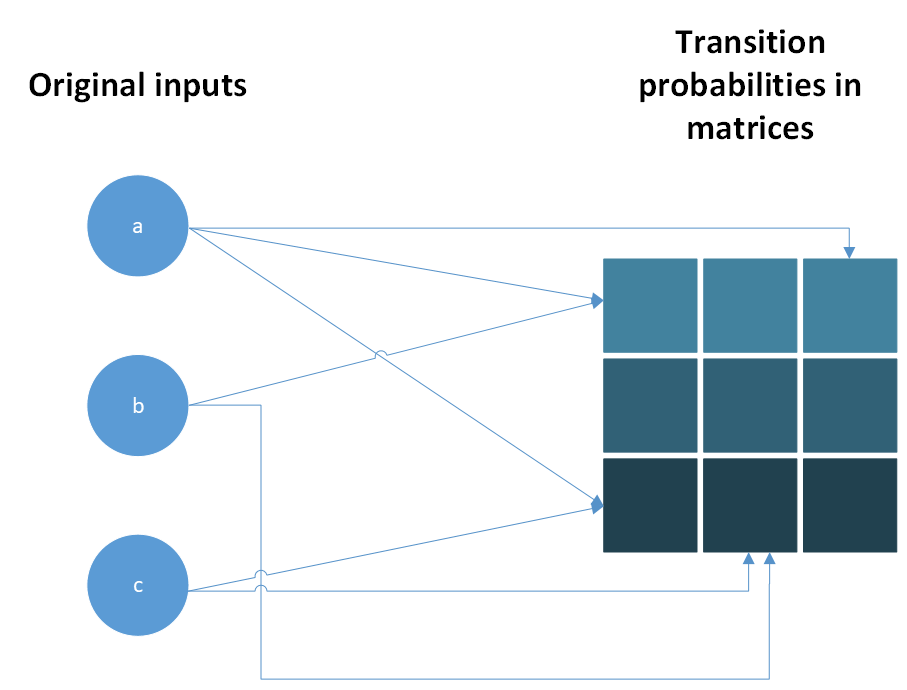
\includegraphics[width=\textwidth]{figures/graph_input_probs}
	\decoRule
	\caption[Dependency graph between inputs and transition probabilities]{We could use graph theory to help optimization considering the dependencies between inputs and the transition probabilities in the matrices.}
	\label{fig:graph_input_probs}
\end{figure}

\subsection{Comments}

\subsubsection*{Pros}
\begin{itemize}
	\item Might help the calibration procedure by exploiting domain knowledge
\end{itemize}

\subsubsection*{Cons}
\begin{itemize}
	\item Overcomplicating the calibration procedure in simple cases
	\item Relationships might not be too complicated
	\item Too vague at this point
\end{itemize}